%Zadání
\section*{Zadání}
\noindent\textit{Vstup: Souvislá polygonová mapa n polygonů \{$P_1, ..., P_n$\}, analyzovaný bod q.}
\vspace{0.8cm}

\noindent\textit{Výstup: $P_i, q \in P_i$.}
\vspace{0.8cm}

\noindent Nad polygonovou mapou implementujete Ray Crossing Algorithm pro geometrické vyhledávání incidujícího polygonu obsahujícího zadaný bod $q$.
\vspace{0.8cm}

\noindent Nalezený polygon graficky zvýrazněte vhodným způsobem (např. vyplněním, šrafováním, blikáním). Grafické rozhraní vytvořte s využitím frameworku QT.
\vspace{0.8cm}

\noindent Pro generování nekonvexních polygonů můžete navrhnout vlastní algoritmus či použít existující geografická data (např. mapa evropských států).
\vspace{0.8cm}

\noindent Polygony budou načítány z textového souboru ve Vámi zvoleném formátu. Pro datovou reprezentaci jednotlivých polygonů použijte špagetový model.
\vspace{1cm}

\subsection*{\textbf{Hodnocení}}
V rámci této úlohy byly řešeny následující kroky:
\begin{table}[htbp]
\resizebox{\linewidth}{!}{%
\begin{tabular}{|l|l|}
\hline
\textbf{Krok}                                                                                  & \textbf{hodnocení} \\ [0.5ex]  \hline\hline
Detekce polohy bodu rozšiřující stavy uvnitř, vně polygonu.                                    &  10 b.              \\ \hline
\textit{Analýza polohy bodu (uvnitř/vně) metodou Winding Number Algorithm.}                    & \textit{+10 b.}    \\ \hline
\textit{Ošetření singulárního případu u Winding Number Algorithm: bod leží na hraně polygonu.} & \textit{+ 5 b.}    \\ \hline
\textit{Ošetření singulárního případu u Ray Crossing Algorithm: bod leží na hraně polygonu.}   & \textit{+ 5 b.}    \\ \hline
\textit{Ošetření singulárního případu obou algoritmů: bod je totožný s vrcholem jednoho či více polygonů.} & \textit{+ 2 b.} \\ \hline
\textit{Zvýraznění všech polygonů pro oba výše uvedené singulární případy.}                    & \textit{+ 3 b.}    \\ \hline
Celkem.                                    
                  &  35 b.              \\ \hline                  
\end{tabular}%
}
\end{table}

%Popis problému
\newpage
\section*{1 Popis a rozbor problému}
\subsection*{1.1 Point Location Problem}
\textit{Point Location Problem} je jedním z nejdůležitějších problémů počítačových aplikací, ve kterých jsou využity geometrické struktury. V rovině je zadána množina n bodů, jež tvoří vrcholy mnohoúhelníků Pj, a dále je určen bod q. Cílem problému je najít takový mnohoúhelník, který obsahuje zmíněný bod q. V praktickém životě clověka jde tedy také o velice důležitou věc, neboť často lidé potřebují znát svoji polohu vzhledem k různým objektům. Point Location Problem bývá často řešen v GIS.
\vspace{0.8cm}

\noindent Zmíněný problém z hlediska automatizace není vůbec snadný, neboť datasety mohou být tvořeny stovkami tisíc i miliony mnohoúhelníků, tudíž jde pak o časově velice náročné algoritmy. Je potřeba nalézt datové struktury a algoritmy, jež umožňují problém řešit efektivně pro konvexní i nekonvexní mnohoúhelníky. Existují dva základní algoritmy, které jsou schopny určit vzájemnou polohu bodu a uzavřených mnohoúhelníků a zároveň jejichž použití je vhodné pro nekonvexní mnohoúhelníky. Jde o \textit{Winding Number Algorithm} a \textit{Ray Crossing Algorithm}, kterým jsou věnovány následující řádky.

%Winding Number
\subsection*{1.2 Winding Number Algorithm}
\textit{Winding Number Algorithm} se používá k analýze polohy bodu pro nekonvexní mnohoúhelníky. Jinak se tomuto algoritmu říká také Metoda ovíjení. Princip spočívá v tom, že pozorovatel stojí v bodě \textit{q}. Pokud bod \textit{q} náleží mnohoúhelníku a pozorovatel chce vidět všechny rohy daného objektu, tak se musí otočit o úhel 360 stupňů. Pakliže však bod \textit{q} danému mnohoúhelníku nenáleží, pak je výše zmíněný úhel menší než 360 stupňů. 

\subsubsection*{1.2.1 Princip algoritmu}
\noindent Výpočet \textit{Winding Number} probíhá tak, že se sečtou všechny úhly $\omega_1$, jež svírá pozorovaný bod $q$ s vrcholy daného polygonu P.\\ 

\begin{equation*}
\Omega (q,P)= \begin{cases}
    1, q  \in P \\
    0, q  \notin P\\
\end{cases}
\end{equation*}\\

 \noindent Abychom zjistili polohu bodu q vzhledem k přímce  $p \approx \overleftrightarrow{P_iP_{i+1}}$,  potřebujeme nejprve spočítat směrový vektor této přímky $q$ a dále také vektor $v$, který spojuje $q$ s $p_i$.\\
 \begin{align}
    \nonumber&\vec{p}=(x_{i+1}-x_i,y_{i+1}-y_i)\\
    \nonumber&\vec{v}=(x_q-x_i,y_q-y_i)
\end{align}\\
Přepišme tyto vektory do matice A a následněme spočtěme její determinant. Výsledný determinant nám určí, zda se pozorovaný bod nachází v levé či pravé polorovině.\\

\begin{equation*}
A=\begin{pmatrix} q_x & q_y \\ v_x & v_y  \end{pmatrix}
\end{equation*}\\

\begin{equation*}
det(A) = (q_x*v_y)-(q_y*v_x)
\end{equation*}\\

\noindent Pokud se bod $q$ nachází v levé polorovině ($\sigma_l$), pak je úhel orientován ve směru hodinových ručiček. Avšak u pravé poloviny ($\sigma_r$) je to přesně naopak a výsledná hodnota $\Omega$ vychází záporná. Výsledek je následně uváděn jako celkový počet oběhů, tedy násobky $2 \pi$.
\vspace{0.8cm}

\begin{equation*} 
\text{det}\begin{cases} < 0, & \text{bod \( q \) leží vpravo od přímky ($\sigma_r$)} \\ > 0,& \text{bod \( q \) leží vlevo od přímky ($\sigma_l$)} \\ = 0 , & \text{bod \( q \) leží na přímce} \end{cases}
\end{equation*}
\vspace{0.8cm}

\noindent Výhodou tohoto algoritmu je efektivita, neboť pro výpočet stačí pouze znát souřadnice bodu a vrcholů polygonu. Není tedy třeba provádět žádné složité geometrické operace. Nevýhodou Winding Number může být citlivost na orientaci hran. Pokud jsou totiž hrany polygonu zadané ve špatném směru, algoritmus může poskytnout chybné výsledky.

%Pseudokód algoritmu Winding Number
\subsubsection*{1.2.2 Pseudokód metody Winding Number}
\begin{algorithm}[H] 
    \caption {\textit{Winding Number}}
    \begin{algorithmic}[1]
        \State  $\varOmega$ = 0, tolerance $\epsilon$       \Comment{Inicializace sumy úhlu a tolerance}
        \State \textbf{for} všechny vrcholy v polygonu:
        \State \indent \textbf{if} bod je vrcholem:
         \State \indent\indent \textbf{return} -1    \Comment{Bod leží na hraně}
        \State \indent spočti determinant        
        \State \indent urči úhel $\omega$ mezi $q$ a $p_i$ a $p_{i+1}$
        \State \indent \textbf{if} determinant > 0:
        \State \indent  \indent $\varOmega$ += $\omega$       \Comment{Bod leží v levé polorovině}
        \State \indent \textbf{if} determinant < 0:
        \State \indent \indent $\varOmega$ -= $\omega$             \Comment{Bod leží v pravé polorovině}
        \State \indent {\textbf{if}} determinant == 0 {\textbf{and}} $\omega$ > $\pi - \epsilon$ :

        \State \indent\indent \textbf{return} -1 \Comment{Bod leží na hraně}
        
        \State \textbf{if} $|\varOmega| - 2\pi < \epsilon$:
        \State \indent\textbf{return} 1\Comment{Bod leží uvnitř polygonu}
        \State   \textbf{return} 0\Comment{Bod leží vně polygonu}
    \end{algorithmic}
\end{algorithm}

%Ray Crossing
\subsection*{1.3 Ray Crossing Method}

\textit{Ray Crossing Method}, často označovaný také jako \textit{Ray Casting Algorithm}, v češtině \textit{paprskový algoritmus} představuje snadnou metodu řešení \textit{point in polygon} problému pro nekonvexní mnohoúhelníky. Metoda určuje vzájemný vztah polygonu a zkoumaného bodu na základě počtu průsečíků, které protíná polopřímka (paprsek) vedená daným bodem. Pokud je počet průsečíků lichý, tak zkoumaný bod náleží danému mnohoúhelníku. Avšak pokud byl zjištěn sudý počet průsečíků, tak bod leží mimo zkoumanou oblast. U tohoto algoritmu ale musíme dávat pozor na singulární případy, kdy dochází k problematickým situacím.

\subsubsection*{1.3.1 Princip algoritmu}
Nejprve vyberme bod pro který chceme zjistit, zda se nachází uvnitř nebo vně polygonu $P$. Tento bod označme jako $q$. Bodem $q$ je vedena polopřímka $r$ \textit{(ray)}, přičemž platí:\\

\begin{equation*}
r(q):y=y_q
\end{equation*}\\
Poté jednoduše vypočteme počet průsečíků - tedy kolikrát paprsek protne hrany polygonu. Pokud je počet průsečíků lichý, bod \textit{q} leží uvnitř polygonu; pokud je sudý, leží vně, tedy: 

\begin{equation*}
k\%2=\begin{cases}
    1, \quad q  \in P\\\textbf{}
    0, \quad q  \notin P\\
    \end{cases}
\end{equation*}\\

\noindent Princip algoritmu Ray Crossing je poměrně snadný, problém však nastává ve chvíli, prochází-li přímka \textit{r} některým z vrcholů polygonu, nebo je-li totožná s nějakou jeho hranou. Pro tyto situace je možné využít modifikaci algoritmu Ray Crossing s redukcí ke \textit{q}. Při této úpravě dochází k posunutí počátku do bodu \textit{q}. Aby byl algoritmus schopen rozpoznat, zda se bod \textit{q} nachází na hrané polygonu, je přímka $r$ dále rozdělena na dvě polopřímky, přičemž jedna má orientaci levostrannou $r_1$ a druhá pravostrannou $r_2$. V situaci, kdy se počet průsečíků $k_l$ a $k_r$ s polopřímkami $r_1$ a $r_2$ neshoduje, znamená to, že bod $q$ leží na hraně polygonu $P$. Bod $q$ je porovnáván se souřadnicemi všech vrcholů polygonu. Jsou-li souřadnice bodu $q$ totožné se souřadnicemi nějakého z vrcholů, leží bod $q$ na vrcholu mnohoúhelníku $P$. I při této variantě metody \textit{Ray Crossing} platí, že je-li počet průsečíků $k_r$ nacházejících se na polopřímce $r_1$ lichý, bod leží uvnitř polygonu $P$.

%Pseudokód algoritmu Ray Crossing
\subsubsection*{1.3.2 Pseudokód metody Ray Crossing}
\begin{algorithm}[H] 
    \caption {\textit{Ray Crossing}}
    \begin{algorithmic}[1]
        \State $k_l$ = 0, $k_r$ = 0                           \Comment{Inicializace průsečíků pro levou a pravou polorovinu}
         \State \textbf{for} všechny vrcholy v polygonu:
         \State \indent \textbf{if} bod je
         vrcholem:
         \State \indent\indent \textbf{return} -1    \Comment{Bod leží na hraně}  
          \State \indent \textbf{if} $y_i == y_{i+1}$: \Comment{Kontrola vodorovných hran} 
          \State \indent \indent \textbf{continue}
        \State \indent vypočti $x$ souřadnice průsečíku $x_m$       
        \State \indent \textbf{if} $(y_i < 0) \neq (y_{i+1}<0)$ \textbf{and} $x_m<0$: \Comment{Levostranný paprsek}        
        \State \indent \indent  inkrementuj počet průsečíků $k_l$        
        \State \indent \textbf{if} $(y_i>0) \neq (y_{i+1}>0)$ \textbf{and} $x_m>0$: \Comment{Pravostranný paprsek}
        \State \indent \indent inkrementuj počet průsečíků $k_r$

        \State \textbf{if} $k_r\%2 = 1$:
        \State  \indent \textbf{return}: 1\Comment{Bod leží uvnitř polygonu}   
        \State \textbf{if} $(k_l + k_r) \%2  \neq 0$:
        \State  \indent \textbf{return} -1\Comment{Bod leží na hraně}             
        \State  \textbf{return} 0\Comment{Bod leží vně polygonu}
    \end{algorithmic}
\end{algorithm}

%Vlastní aplikace
\newpage
\subsection*{2 Vlastní aplikace}

%Vstupní data
\subsubsection*{2.1 Vstupní data}

\noindent Jako vstupní data byla vybrána polygonová vrstva městských částí Prahy. Tato data jsou v Křovákově zobrazení. Vzniklá aplikace umožňuje práci se soubory ve formátu shapefile. U aplikace jsou uloženy námi vybraná testovací data ve zmíněném formátu.

%Grafické rozhraní
\subsubsection*{2.2 Grafické rozhraní aplikace}
\noindent Grafické rozhraní aplikace bylo vytvořeno v prostředí \textit{Qt creator}. Po spuštění aplikace se otevře okno, v jehož horní části se nachází menu s jednotlivými funkcemi. V záložce \textit{File} si uživatel může vybrat z dvou různých funkcí. Po stisknutí \textit{Open} se otevře nové okno, ve kterém je možné vybrat data ve formátu \textit{shapefile}, která jsou následně vykreslena na rozsáhlou volnou plochu v aplikaci. Pokud uživatel stiskne \textit{Exit}, bude aplikace uzavřena. Grafické rozhraní aplikace je znázorněna na obrázku 1.\\

\begin{figure}[H]
    \centering
    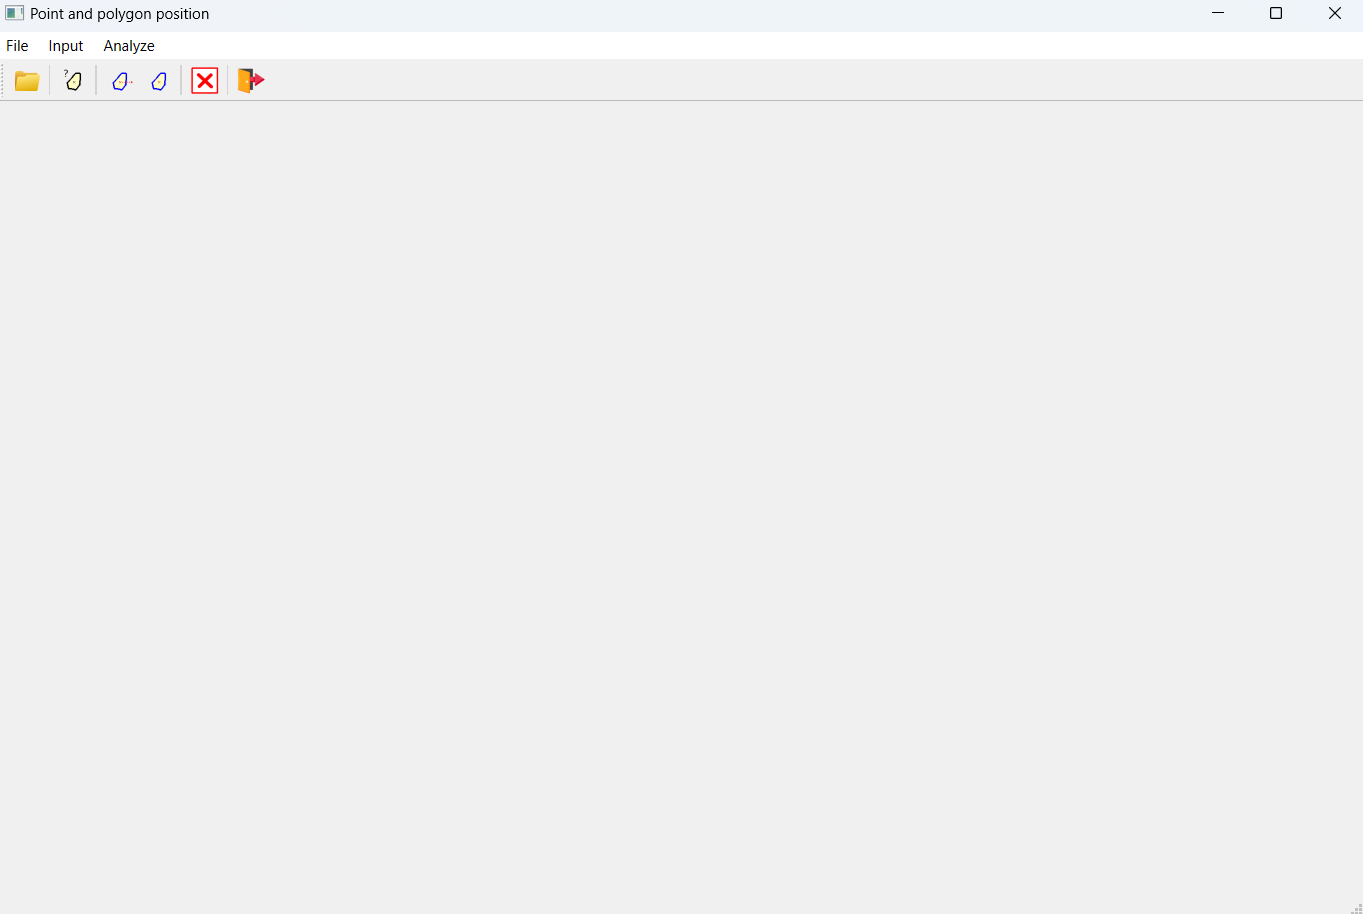
\includegraphics[width=0.65\linewidth]{graficke_rozhrani.png}
    \caption{Grafické rozhraní aplikace}
    \label{fig:enter-label}
\end{figure}

\noindent Pokud chce uživatel nakreslit bod, stačí pouze kliknout levým nebo pravým tlačítkem myši na volnou plochu a červenou barvou se vykreslí bod. V záložce \textit{Input} si může uživatel vybrat funkci \textit{Clear}, pomocí které jsou smazána všechna nahraná data (tedy polygony i bod).\\

\noindent Další záložkou naší aplikace je \textit{Analyze}, kde jsou v nabídce funkce \textit{Ray Crossing Algorithm} a \textit{Winding Number Algorithm}. Zde si uživatel může zvolit pomocí kterého algoritmu chce analyzovat polohu svého vytvořeného bodu vůči polygonové vrstvě. Po stisknutí tlačítka zvoleného algoritmu se modrou barvou označí polygon, ve kterém daný bod leží. Tento jev je znázorněn na následujícím obrázku.

\begin{figure}[H]
    \centering
    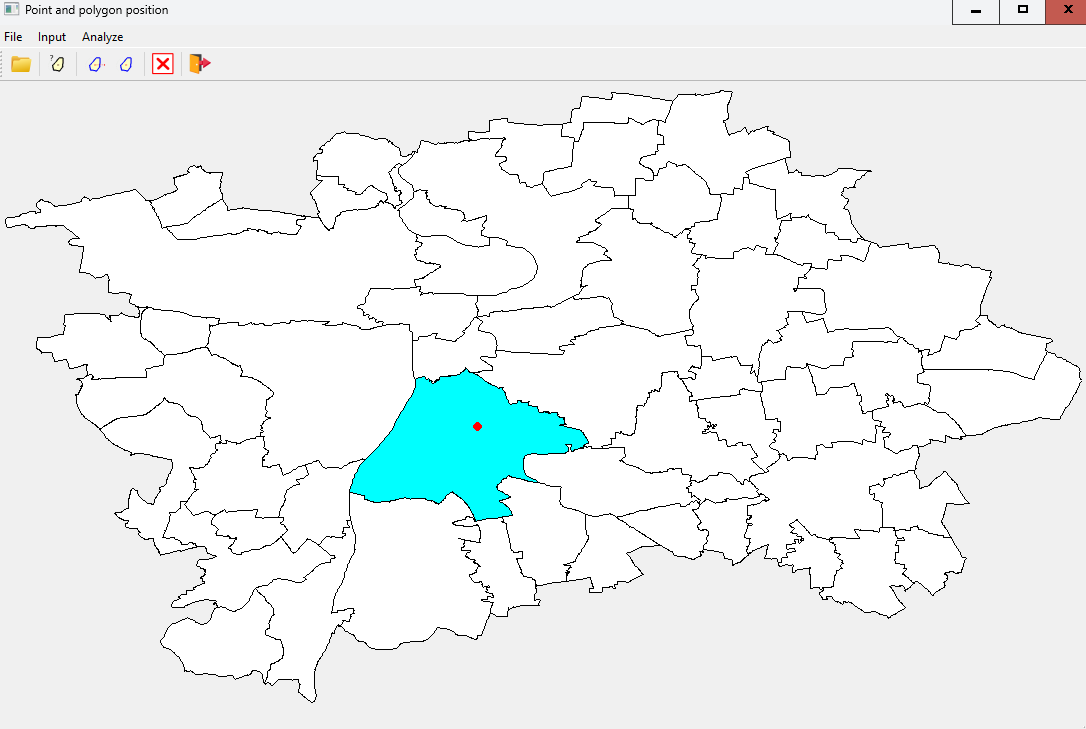
\includegraphics[width=0.65\linewidth]{bod_uvnitr_polygonu.png}
    \caption{Bod ležící uvnitř polygonu}
    \label{fig:enter-label}
\end{figure}

\noindent Dále bylo také ošetřeno, aby při poloze bodu na hraně či vrcholu polygonu byly označeny všechny polygony, na jejichž hranicích bod leží. Zmíněná situace je znázorněna na obrázku 3, kde bod leží na hraně třech polygonů.

\begin{figure}[H]
    \centering
    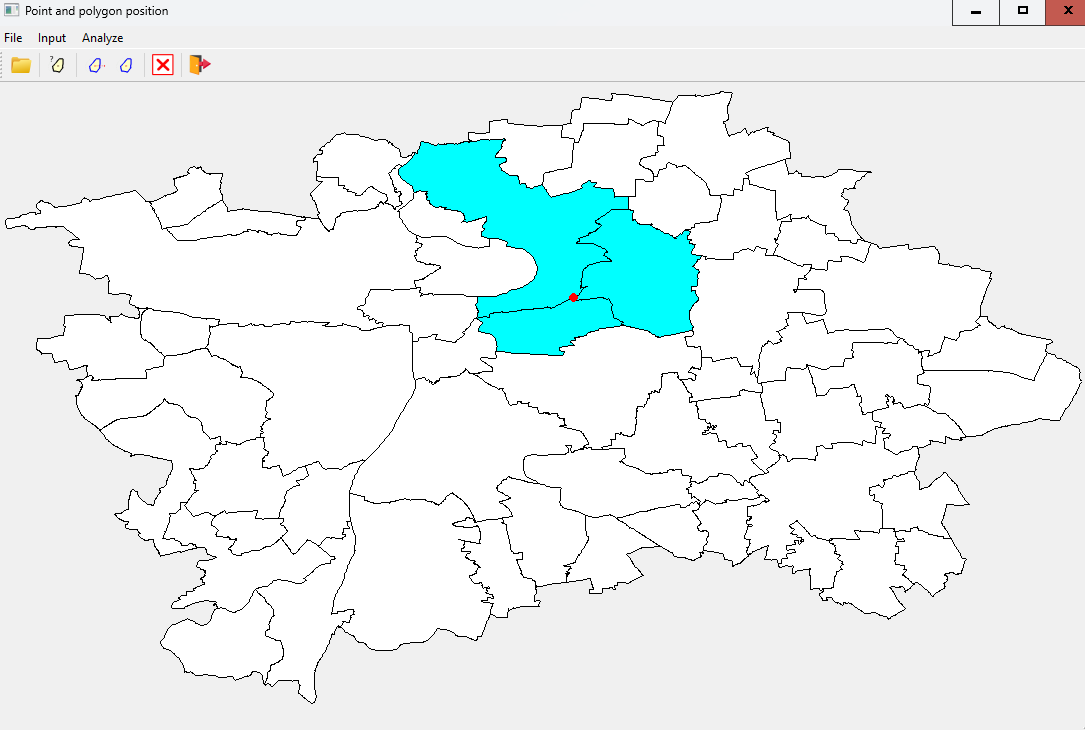
\includegraphics[width=0.65\linewidth]{bod_na_hrane.png}
    \caption{Bod ležící na hraně více polygonů}
    \label{fig:enter-label}
\end{figure}

\noindent Na horním panelu jsou také umístěny ikony, pomocí kterých může uživatel rychleji vyvolat požadovanou funkci. Tyto ikony odpovídají funkcím, ketré jsou v jednotlivých záložkách nad nimi. Konkrétně jde tedy zleva o následující ikony: \textit{Open file}, \textit{Input point}, \textit{Ray Crossing Algorithm}, \textit{Winding Number Algorithm}, \textit{Clear data} a \textit{Close application}.

%Dokumentace
\subsubsection*{2.3 Dokumentace programu}

\noindent Program byl vytvořen v prostředí \textit{Visual Studio Code} v programovacím jazyce Python. Součástí programu jsou následující soubory: \textit{mainform.py, draw.py, algorithms.py}. Složka \textit{icons} obsahuje obrázky s ikonami nezbytné pro přehledné fungovaní aplikace.\\

%Třída mainform
\noindent
\textbf{Třída mainform}\\
Třída \textit{mainform} je určena k nastavení uživatelského rozhraní aplikace a propojení s metodami definovanými v ostatních třídách. Konkrétně tato třída zabezpečuje inicializaci okna aplikace, panelu nástrojů, vrchní lišty a dále také jednotlivých ikon a tlačítek. Celkem je v \textit{mainform} obsaženo sedm metod, z nichž dvě ({\fontfamily{qcr}\selectfont
setupUi(MainWindow)} a {\fontfamily{qcr}\selectfont
retranslateUi(MainWindow)}) vznikly automaticky po vytvoření prostředí v QtCreator. Dále jsou zde následující nové metody:
\begin{itemize}
    \item {\fontfamily{qcr}\selectfont
openClick()}: otevírá soubor ve formátu shapefile a načítá ho do proměnné
    \item {\fontfamily{qcr}\selectfont
handleClick(algorithm)}: analyzuje polohu bodu q vůči polygonu
    \item {\fontfamily{qcr}\selectfont
windingNumberClick()}: nastavuje Winding Number jako algoritmus pro analýzu polohy bodu
    \item {\fontfamily{qcr}\selectfont
rayCrossingClick()}: nastavuje Ray Crossing jako algoritmus pro analýzu polohy bodu
    \item {\fontfamily{qcr}\selectfont
clearClick()}: maže nahrané polygony a bod
\end{itemize}

%Třída draw
\noindent\\
\textbf{Třída draw} \\
Třída \textit{draw} zajišťuje grafické rozhraní, slouží tedy k vykreslení prostorových dat a ovládání aplikace. V této třídě jsou obsaženy následující metody:
\begin{itemize}
    \item {\fontfamily{qcr}\selectfont
mousePressEvent(e:QMouseEvent)}: odečítá aktuální souřadnice kurzoru myši
    \item {\fontfamily{qcr}\selectfont
paintEvent(e:QPaintEvent)}: vykresluje body a polygony na plátno
    \item {\fontfamily{qcr}\selectfont
getQ()}: vrací souřadnice bodu
    \item {\fontfamily{qcr}\selectfont
getPolygons()}: vrací seznam vstupních polygonů
    \item {\fontfamily{qcr}\selectfont
getPol()}: vrací analyzovaný polygon (analyzované polygony)
    \item {\fontfamily{qcr}\selectfont
clearPol()}: odstraňuje veškeré kresby na plátně
    \item {\fontfamily{qcr}\selectfont
setHighlightedPolygons(indices)}: nastavuje seznam indexů polygonů, které mají být zvýrazněny
    \item {\fontfamily{qcr}\selectfont
loadDataAndRescalePolygons(width, height)}: načítá prostorová data a roztahuje je v závislosti na velikosti grafického okna
\end{itemize}

%Třída algorithms
\newpage
\noindent
\textbf{Třída algorithms}\\
Třída \textit{algorithms} obsahuje metody, které jsou detailně popsány v předchozí kapitole, která se detaině věnuje použitým algoritmům. Tato třída je tedy tvořena následujícími metodami:
\begin{itemize}
    \item {\fontfamily{qcr}\selectfont
rayCrossing (q, pol)}: pomocí algoritmu Ray Crossing analyzuje polohu bodu q vůči polygonu pol
    \item {\fontfamily{qcr}\selectfont
windingNumber (q, pol)}: pomocí algoritmu Winding Number analyzuje polohu bodu q vůči polygonu pol
\end{itemize}

%Závěr
\newpage
\subsection*{3 Závěr}
\noindent V této úloze byla vytvořena aplikace, která na základě uživatelem zvoleného algoritmu analyzuje polohu bodu vůči polygonům. Konkrétně si uživatel může vybrat mezi \textit{Ray Crossing} a \textit{Winding Number}, což jsou algoritmy schopné řešit problém bodu a polygonu pro nekonvexní mnohoúhelníky. Aplikace dokáže také vyřešit singularity, tedy že vybraný bod leží na hraně či vrcholu polygonu.\\

\noindent Možným zlepšením aplikace by mohla úprava, aby byla schopna vyřešit i úlohu pro polygony s dírami. Dalším vylepšením by určitě bylo nahrání souboru v jiném formátu, neboť současná aplikace dokáže nahrát pouze data ve formátu \textit{shapefile}. Užitečné by bylo, kdyby do aplikace šla nahrát data například formátů \textit{JSON} nebo \textit{GeoJSON}. Uživatelé by také určitě uvítali, kdyby si v aplikaci mohli přibližovat a oddalovat, což by jim umožnilo přesnější umístění bodu. Tato vlastnost by aplikaci také výrazně vylepšila.

%Zdroje
\newpage
\subsection*{4 Zdroje}

\noindent BAYER, T. (2024): Point Location Problem. Prezentace pro předmět Algoritmy počítačové kartografie, dostupné z: https://web.natur.cuni.cz/~bayertom/index.php/teaching/algoritmy-pocitacove-kartografie (cit. 21. 3. 2024).\\

\noindent HECKBERT, P. S. (1994). Graphics Gems IV. Morgan Kaufmann.\\

\noindent HUANG, C. W., SHIH, T. Y. (1997): On the complexity of Point-in-Polygon Algorithms. Computers and Geosciences, 23 (1), 109-118.\\

\noindent ROURKE, O. J. (1998): Computational Geometry in C. Cambridge University Press, Cambridge.






